
\chapter{Phylogenetic Clustering (Phyloclustering)}
\label{chp:phyloclustering}


\inspire{What one man can invent another can discover.}{Sherlock Holmes}


\section{Introduction}

Phylogenetic Clustering (Phyloclustering)\index{phyloclustering}
discovers population structure based on information of DNA/RNA sequences
by combining two inventions: model-based clustering with evolutionary
models~\citep{Chen2011a}.
Note that what speaking here, regarding to ``evolutionary'',
is a mathematical/statistical model to interpret biological targets.
Neither religion nor theology is involved. 

In an over simplified case, suppose a sequence is composed by four nucleotides
$\mS = \{\colorA, \colorG, \colorC, \colorT\}$.
Assume a sequence
$\bx_n = \{x_{n1}, x_{n2},\ldots, x_{nL}\} \in \mS$
has $L$ loci (positions ordered) and is observed from a population, but
may have $K$ subpopulations that similar sequence patterns are expected
within each common subpopulation.
Each subpopulation is represented by a common center sequence
$\bmu_k = \{\mu_{k1}, \mu_{k2},\ldots, \mu_{kL}\} \in \mS$
which may or may not hypothetically exit in population and has to be
determined.
Therefore, each sequence has a probability mutated/evolved from any
center sequence. The higher the probability, the closer (more similar)
to the center sequence. This bold assumption may be invalid to and even violate
traditional phylogeny construction and evolutionary research, but it is
a comparative way to reconstruct population structures totally
based on the discovered facts of observed data.

The evolutionary model is based on a continuous time Markov chain
(CTMC)\index{continuous time Markov chain}\index{CTMC} model
on a state space $\mS$
that the mutation process is characterized by
an instantaneously rate matrix $\bQ$ with dimension $4\times 4$,
i.e. rate at scale of tiny mutation time $t\rightarrow 0$.
We use the following steps to construct the likelihood function
as introduced in Chapter~\ref{chp:likelihood}:
\begin{enumerate}
\item
Given the above setting,
the mutation chance from a nucleotide $x$ to a nucleotide $y$ in time $t$ is
\begin{equation}
\Prob_{x, y}(t) = e^{\bQ_{x, y}t}
\label{eqn:e_Qt}
\end{equation}
for all $x, y \in \mS$.

\item
Assume each locus is mutated independently, then the mutation chance
(the transition probability) from $\bmu_k$ to $\bx_n$ in time $t$ is
$$
p_{\bmu_k, \bx_n}(t) = \prod_{l = 1}^L \Prob_{\mu_{kl}, \bx_{nl}}(t)
$$
for all $\bmu_{kl}, \bx_{nl} \in \mS$.

\item
Suppose there are $K$ subpopulations with mixing proportion $\eta_k$'s, then
the mutation chance from a sequence $\bmu_k$ to a sequence $\bx_n$ is
\begin{equation}
f(\bx_n; \btheta_K) = \sum_{k = 1}^K \eta_k p_{\bmu_k, \bx_n}(t)
\label{eqn:phyclust_mixture}
\end{equation}
where $\btheta_K = \{\eta_1, \eta_2, \ldots, \eta_{K-1},
                     \bmu_1, \bmu_2, \ldots, \bmu_{K}, \bQ, t\}$
are unknown and to be determined.
For simplicity, assume $\bQ$ and $t$ are identical across $K$ subpopulations.
Denote the distribution $\mF(\btheta_K)$ of the density function
$f(\bx_n; \btheta_K)$ for $\bx_n$.

\item
Suppose observed $N$ sequences $\bx = \{\bx_1, \bx_2, \ldots, \bx_N\}$
(each has $L$ loci)
independently and identically selected from unknown $K$ subpopulations
with mixing proportion $\boldeta$ to be estimated,
then the likelihood is
$$
L(\btheta_K; \bx) = \prod_{n = 1}^N f(\bx_n; \btheta_K).
$$
See Section~\ref{sec:likelihood_introduction} for construction.

\item
In short, the log likelihood is
\begin{eqnarray}
\log L(\btheta_K; \bx)
  & = & \sum_{k = 1}^K \log f(\bx_n; \btheta_K) \nonumber \\
  & = & \sum_{k = 1}^K \log
        \left[
        \sum_{k = 1}^K \eta_k p_{\bmu_k, \bx_n}(t)
        \right] \nonumber \\
  & = & \sum_{k = 1}^K \log
        \left[
        \sum_{k = 1}^K \eta_k
        \left(
        \prod_{l = 1}^L \Prob_{\mu_{kl}, \bx_{nl}}(t)
        \right)
        \right] \nonumber \\
  & = & \sum_{k = 1}^K \log
        \left[
        \sum_{k = 1}^K \eta_k
        \left(
        \prod_{l = 1}^L e^{\bQ_{\mu_{kl}, \bx_{nl}}t}
        \right)
        \right].
\label{eqn:phyclust_mixture_logl}
\end{eqnarray}

\end{enumerate}

Equation~(\ref{eqn:phyclust_mixture}) has similar structure
as Equation~(\ref{eqn:gaussian_mixture}). Therefore, the
EM algorithm~\citep{Dempster1977}\index{Algorithm!EM}
can be applied to maximize Equation~(\ref{eqn:phyclust_mixture_logl})
as maximize Equation~(\ref{eqn:gaussian_mixture_logl}).
Except the parameter space $\bTheta_K$ of
Equation~~(\ref{eqn:phyclust_mixture_logl}) where $\btheta_K$ belongs to
is neither continuous nor discrete space since $\bx_n$ and $\bmu_k$ are
in a categorical space which yields a very different E- and M-steps.


\section{The \pkg{phyclust} Package}
\label{sec:phyclust}

The \pkg{phyclust}~\citep{Chen2011a}
is an \proglang{R} package fully implements
phyloclustering with different configurations, EM algorithms, and
incorporating several useful tools such as \pkg{ms}~\citep{Hudson2002}
for simulating phylogeny and \pkg{seq-gen}~\citep{Rambaut1997}
for simulating sequence with vary mutations based on phylogenies.
The \pkg{phyclust} also provides functions for re-sampling sequences from
predicted models for determining an appropriate number of subpopulations.
Those functions are particular useful for Sections~\ref{sec:bootstrap}
and~\ref{sec:task_pull}.

The \pkg{phyclust} package has several example datasets which is initialed by
several longitudinal animal studies on Equine Infectious Anemia
Virus (EIAV)~\citep{Leroux2004}\index{EIAV}.
The EIAV is a lentivirus that
infects equine and causes Equine Infectious Anemia (EIA), and it is similar
to Human Immunodeficiency Virus (HIV) infects human and causes Acquired
Immunodeficiency Syndrome (AIDS).
Figure~\ref{fig:retrovirus}~\citep{Weiss2006}
shows a phylogeny of several relative lentivirus
in the retrovirus family, it also shows the closeness of EIAV and HIV which
makes the possible to build an animal model based on EIAV and to study
viral transmission mechanism further in HIV.

\begin{figure}[h!tb]
\centering
 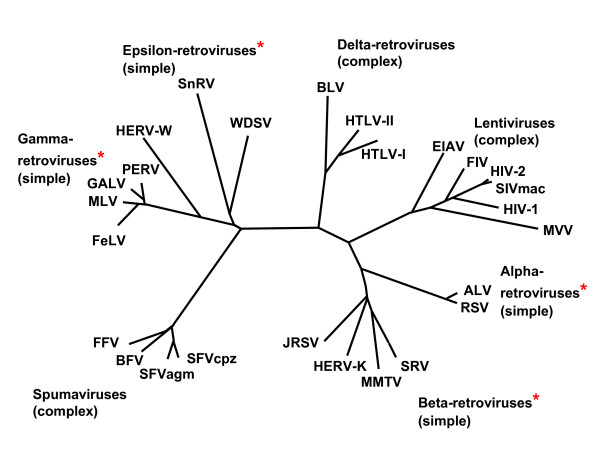
\includegraphics[width=5.5in]{pbdDEMO-include/pics/Phylogeny_of_Retroviruses}
\caption{Retrovirus phylogeny originated from~\citet{Weiss2006}.}
\label{fig:retrovirus}
\end{figure}

The disease EIA progresses as the immune system
response to the viruses population change in blood which is collected
over time and generations. Part of blood samples associated with fever cycles
are sequenced to identify highly mutable coding regions with several
overlapping reading frames. Immune system response to new mutants of EIAV and
trigger fever as a major signal and symptom of EIA. Therefore, the
sequences and regions then can be associated with disease progresses for
further analysis. Identify population structures is the critical step for
understanding the mutation patterns and designing better medicine or vaccine.

We perform phyloclustering on an example dataset,
{\it Pony 524}~\citep{Carpenter2011},\index{Data!Pony 524}
which is given in Figure~\ref{fig:eiav}.
See~\citet{Baccam2003} for more about the studies and stories of infected
horses.
It plots the example dataset where $N = 146$ EIAV sequences
are in y-axis and $L = 405$ loci in x-axis.
The top row is the consensus sequence, and only mutation sites are spotted
for 146 sequences. Colors represent $\colorA$, $\colorC$, $\colorG$, and
$\colorT$ nucleotides. Three clusters fitted by a CTMC model are shown where
common mutation locations and types are grouped by colored spots.
\begin{figure}[h!tb]
\centering
 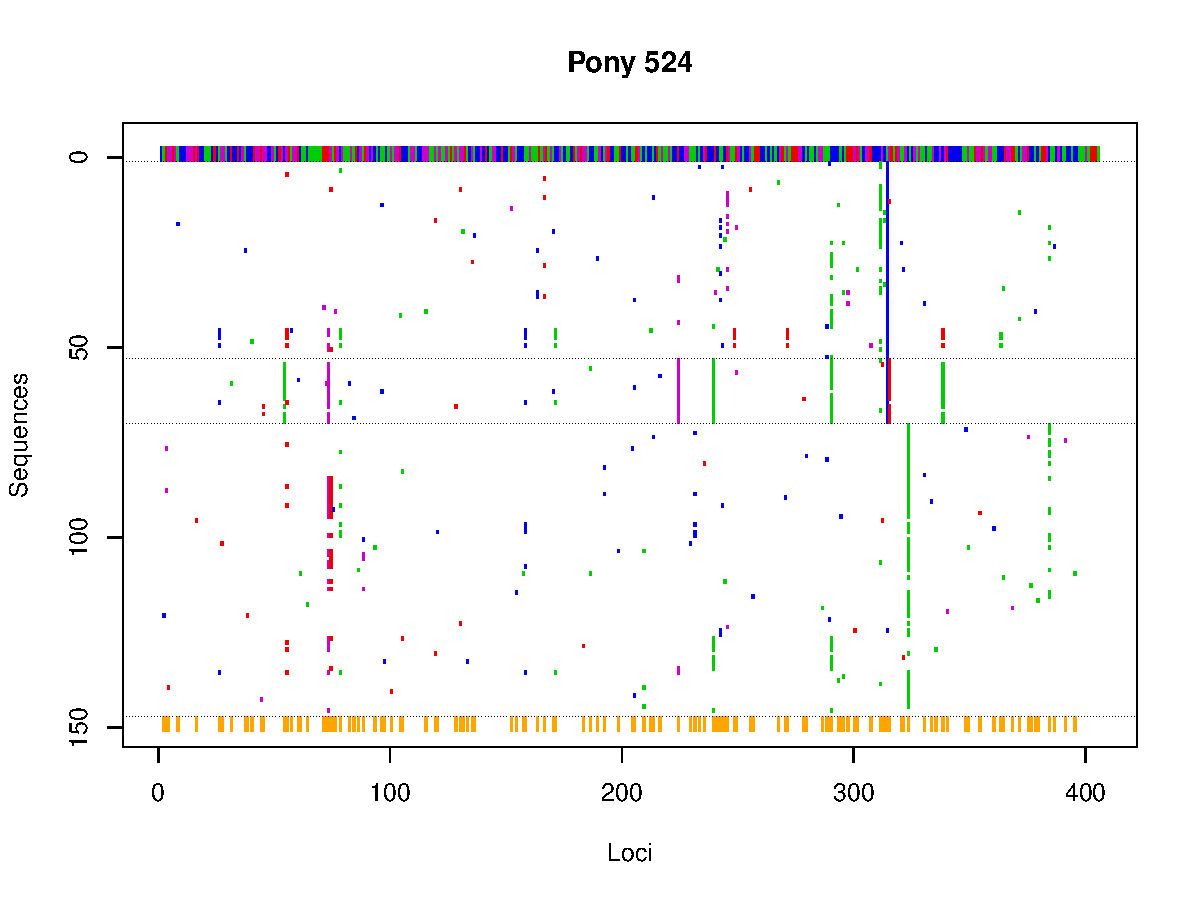
\includegraphics[width=6.5in]{pbdDEMO-include/pics/pony524}
\caption{146 EIAV sequences of {\it Pony 524} in three clusters.}
\label{fig:eiav}
\end{figure}




\section{Bootstrap Method}
\label{sec:bootstrap}

``How many clusters are appropriate for the data?'' is a typical question
to any good scientists. There are several ways trying to infer this from
data in statistics via hypothesis testing. For example,
$H_0: K = 2 \mbox{ v.s. } H_a: K = 3$ or more generally
$H_0: K = K^\prime \mbox{ v.s. } H_a: K = K^*$ for any $K^\prime < K^*$.
In mixture models, the nested parameter space is inappropriate, hence,
the LRT introduced in Section~\ref{sec:lrt} may not appropriate.

The Bootstrap method~\citep{Efron1979}\index{bootstrap}
may provide an adequate solution to
rebuild an asymptotic distribution for the likelihood ratio (LR).
``Asymptotic'' means ideally large sample size property.
The bootstrap method is a re-sampling technique\index{re-sampling technique}
based on Monte Carlo\index{Monte Carlo} property
either from data (non-parametric)
or from model (parametric) to form a distribution for a testing statistics.
Here we need a distribution such as a
hypothetically chi-squared distribution for LR where the degrees of freedom
are difficult to be determined.
Therefore, we may obtain a p-value by comparing LR to this distribution
rather than deriving an asymptotic distribution from LRT.

Phyloclustering which uses a mixture models with unusual parameter space
which is also particular suitable to apply the bootstrap methods to determine
an appropriate number of subpopulations.
For given data $\bX$ and hypothetical $K^\prime$ and $K^*$,
we may perform parametric bootstrap as the next.
\begin{enumerate}[label=Step \arabic*:]
\item
Based on $\bX$,
obtain MLEs $\hat{\btheta}_{K^\prime\,ML}$ and $\hat{\btheta}_{K^*\,ML}$
under $\bTheta_{K^\prime}$ and $\bTheta_{K^*}$, respectively.

\item
Compute and let
$
  \hat{\lambda} :=
  -2\log \hat{\Lambda}
  (\hat{\btheta}_{K^\prime\,ML},
   \hat{\btheta}_{K^*\,ML}; \bX).
$

\item
Sample new data $\bX^{(b)}$ from $\mF(\hat{\btheta}_{K^\prime\,ML})$.

\item
Based on $\bX^{(b)}$,
obtain MLEs $\hat{\btheta}^{(b)}_{K^\prime\,ML}$ and
$\hat{\btheta}^{(b)}_{K^*\,ML}$
under $\bTheta_{K^\prime}$ and $\bTheta_{K^*}$, respectively,
via the EM algorithm.

\item
Compute and let
$
  \lambda^{(b)} :=
  -2\log \hat{\Lambda}
  (\hat{\btheta}^{(b)}_{K^\prime\,ML},
   \hat{\btheta}^{(b)}_{K^*\,ML}; \bX^{(b)}).
$

\item
Repeat Steps 3 to 5 for $B$ times, collect and let
$\mF^{(B)}(\lambda) := \{\lambda^{(1)}, \lambda^{(2)}, \ldots, \lambda^{(B)}\}$
which is an approximation to $\mF(\lambda)$,
the distribution of $\lambda$, as $B$ large enough.

\item
If $\hat{\lambda}$ is greater than $q_{\mF^{(B)}(\lambda)}(0.95)$, then
we reject the $K^\prime$ model under $0.05$ level of type I error
with $B$ bootstrap samples.

\end{enumerate}
Unlike LRT of Section~\ref{sec:lrt}, note that
$\hat{\btheta}_{K^*\,ML}$ in Step 1 and
$\hat{\btheta}^{(b)}_{K^*\,ML}$ in Step 4
are MLEs in space $\bTheta_{K^*}$ rather than the spaces
$\bTheta_{K^\prime} \cup \bTheta_{K^*}$ nor $\bTheta_{K^\prime + K^*}$,
which means no guarantee the estimators are the MLEs of larger spaces.
This makes the general LRT invalid for mixture models, therefore, other
information criteria such as AIC~\citep{aic}\index{AIC} are also questionable
for determining a suitable number of clusters.
Parametric or non-parametric bootstraps are other robust methods 
to verify and provide a suggestion.
See \citet{Chen2011a} for more simulation studies of this approach via
\pkg{phyclust}.




\section{Task Pull Parallelism}
\label{sec:task_pull}

Obviously, Step 4 will be computationally intensive as $B$ increased,
and no guarantee that each of $b = 1,2,\ldots, B$ bootstrap samples
will take similar time at obtaining MLEs. It may be possible to parallelize
the EM algorithm fully in SPMD\index{Parallelism!SPMD} such as
Section~\ref{sec:parallel_model_based_clustering},
however, this step is still a bottleneck of whole computation in general.

The task parallelism\index{Parallelism!task parallelism}
as mention in Exercise~\ref{ch2:exercise:2}
is one way to solve the problem by simply divided jobs equally likely
to all processors.
This is probably an optimal solution for equal loading jobs
in homogeneous computing environment. However, it
will be a terrible solution for unbalance loading jobs or in-homogeneous
computing environment, such as
bootstrap methods introduced in Section~\ref{sec:bootstrap}.
Note that there are also some drawbacks for task parallelism:
\begin{itemize}
\item
it requires one processor to handle job controls as the role of manager in
manager/workers programming paradigm,\index{Parallelism!manager/works paradigm}
\item
the code is not obviously and difficult to debug or generalize,
\item
the code requires further reordering for returned results, and
\item
jobs may break in workers which can cause crash of entire computation.
\end{itemize}

The website at
\href{http://math.acadiau.ca/ACMMaC/Rmpi/examples.html}{
http://math.acadiau.ca/ACMMaC/Rmpi/examples.html}
has a general view of task parallelism and examples in \pkg{Rmpi}.
Among three task parallel methods, task pull has the best performance and
suit for bootstrap methods.
A simplified example of task pull in SPMD can be found in the \pkg{pbdMPI}
demo via
\begin{lstlisting}
### At the shell prompt, run the demo with 4 processors by
### (Use Rscript.exe for windows system)
mpiexec -np 4 Rscript -e "demo(task_pull,'pbdMPI',ask=F,echo=F)"
\end{lstlisting}
which does the following
\begin{lstlisting}[language=rr,title=Task Pull Example in \pkg{pbdMPI}]
### Initial
library(pbdMPI, quiet = TRUE)

### Examples
FUN <- function(jid){
  Sys.sleep(1)
  jid * 10
}

ret <- task.pull(1:10, FUN)
comm.print(ret)

if(comm.rank() == 0){
  ret.jobs <- unlist(ret)
  ret.jobs <- ret.jobs[names(ret.jobs) == "ret"]
  print(ret.jobs)
}

### Finish
finalize()
\end{lstlisting}
Lines 5 to 8 define a major function to be evaluated on all workers which are
ranks $1$, $2$, and $3$ in this case.
Line 10 prepares 10 jobs from 1 to 10 where jobs can be done by any
available worker. The \code{task.pull()} is actually a combination of two
functions \code{task.pull.workers()} called by all workers and
\code{task.pull.master()} only called by the master by default rank 0.
Lines 13 to 17 extract and summarize all returned results on master.




\section{An Example Using the {\it Pony 524} Dataset}
\label{sec:ex_pony524}

As introduced in Section~\ref{sec:phyclust}, we will fit the $K^\prime = 1$ and
$K^* = 2$ first. Then, we use bootstrap method in Section~\ref{sec:bootstrap}
to find out better number of clusters based on $B = 100$,
i.e. we compare 
$\hat{\lambda} = -2\log \hat{\Lambda}
  (\hat{\btheta}_{1,ML}, \hat{\btheta}_{2\,ML}; \bX)$
to
$\lambda^{(b)} =
  -2\log \hat{\Lambda}
  (\hat{\btheta}^{(b)}_{1\,ML},
   \hat{\btheta}^{(b)}_{2\,ML}; \bX^{(b)})$
with $b = 1, 2, \ldots, B$ bootstrap samples $\bX^{(b)}$ which are generated
from $\hat{\btheta}_{1,ML}$.
The idea here is if one cluster (or non cluster) were suggested from data, then
$\hat{\lambda}$ would have tiny chance located at the tail region of
$\lambda^{(b)}$'s histogram. On the other hand, if $\hat{\lambda}$ did located
at the tail region, then we might say it is not happen randomly and the
evidence is significant to reject one cluster with small error when
comparing with two clusters based on $B$ bootstrap samples.

The whole processes are designed using the task pull method in
Section~\ref{sec:task_pull} to efficiently
complete all likelihood estimations of all bootstrap cases on $4$ processors
($1$ master and $3$ workers).
The demo code for the Pony 524 example can be found with the package demos,
and executed via:
\begin{lstlisting}
### At the shell prompt, run the demo with 4 processors by
### (Use Rscript.exe for windows system)
mpiexec -np 4 Rscript -e "demo(phyclust_bootstrap,'pbdDEMO',ask=F,echo=F)"
\end{lstlisting}

After a long running, this demo should produce an output that looks something
like the following:
\begin{CodeOutput}
K0: 1
Ka: 2
logL K0: -4033.154
logL Ka: -3403.873
LRT: -1258.561
p-value: 0
\end{CodeOutput}
Note that rerun the code again may produce different results since
job assignments to workers are randomly dependent on bootstrap samples.
However, the conclusion should be similar
that $K^\prime = 1$ is rejected under $0.05$ level type I error
using $B = 100$ parametric bootstraps samples.
This may suggest more than one subpopulations exist in this dataset,
and more detail investigation should be conducted.




\section{Exercises}
\label{sec:phyclust_exercise}

\begin{enumerate}[label=\thechapter-\arabic*]

\item
Argue that the instantaneously rate matrix $\bQ$ of Equation~\ref{eqn:e_Qt}
is positive definite. Therefore, argue that the
eigenvlaues decomposition\index{Decomposition!eigenvalues decomposition}
of $\bQ = \bU\bD\bU^{-1}$ exists. Prove that
$e^{\bQ t} = \bU e^{\bD t} \bU^{-1}$. Hence, this an easy way for
computing transition probability $\Prob_{x,y}(t)$.

\item
Argue that $\mF^{(B)}(\lambda)$ is a good approximation to $\mF(\lambda)$
in Step 4 of Section~\ref{sec:bootstrap}.

\item
In Section~\ref{sec:ex_pony524}, we have tested
$H_0: K^\prime = 1$ v.s. $H_a: K^* = 2$.
Change the code to test $H_0: K^\prime = 1$ v.s. $H_a: K^* = 3$ and
$H_0: K^\prime = 2$ v.s. $H_a: K^* = 3$. Drawn conclusions for these tests.

\item
Implement a function \code{task.push()} for task push parallelism utilizing
examples at the website
\href{http://math.acadiau.ca/ACMMaC/Rmpi/examples.html}{
http://math.acadiau.ca/ACMMaC/Rmpi/examples.html}.

\item
Compare the computation time of \code{pbdLapply()}, \code{task.pull()}, and
\code{task.push()} using in SPMD and in $4$ processors.
By testing $H_0: K^\prime = 1$ v.s. $H_a: K^* = 2$
to Pony 524 dataset using bootstrap method
as Section~\ref{sec:ex_pony524}.

\end{enumerate}

